% !TeX root = main.tex

\section{CW 复形的同调}

\subsection{CW 复形及其结构}

与 $ \D^n $ 同胚的几何体称作一个 $ n $--\emph{胞腔}($ n $--cell), 与 $ \B^n $ 同胚的几何体称作一个 $ n $--\emph{开胞腔}. 习惯上记 $ n $--开胞腔为 $ e_n $, $ n $--胞腔为 $ \bar{e}_n $. 特别地, 约定0--胞腔是单点 $ \mathrm{pt} $, 并用 $ e_0 $ 记它.

\begin{Example}
	球面 $ \S^n $ 可以看作是一个 0--胞腔 $ e_0 $ 和一个 $ n $--开胞腔 $ e_n $ 构成的, 这因 $ \S^n $ 去掉北极点 $ N $ 后
	\[
		\S^n\sm N\cong\R^n\cong\B^n\cong e_n.
	\]
	那么多个球面的一点并从胞腔的角度来看是一件非常平凡的事情. $ k $ 个不同维数的球面一点并 $ \S^{n_1}\vee\S^{n_2}\vee\dots\vee\S^{n_k} $ 无非就是 $ e_0,e_{n_1},e_{n_2},\dots,e_{n_k} $ 构成的.
\end{Example}

\begin{Example}[环面和 Klein 瓶]
	环面 $ \T^2 $ 和 Klein 瓶 $ S $ 都可以看作一个 0--胞腔 $ e_0 $, 两个 1--开胞腔 $ e_1^1 $ 和 $ e_1^2 $, 以及一个 2--开胞腔 $ e_2 $ 构成的复形:
	\begin{figure}[htbp]
		\centering
		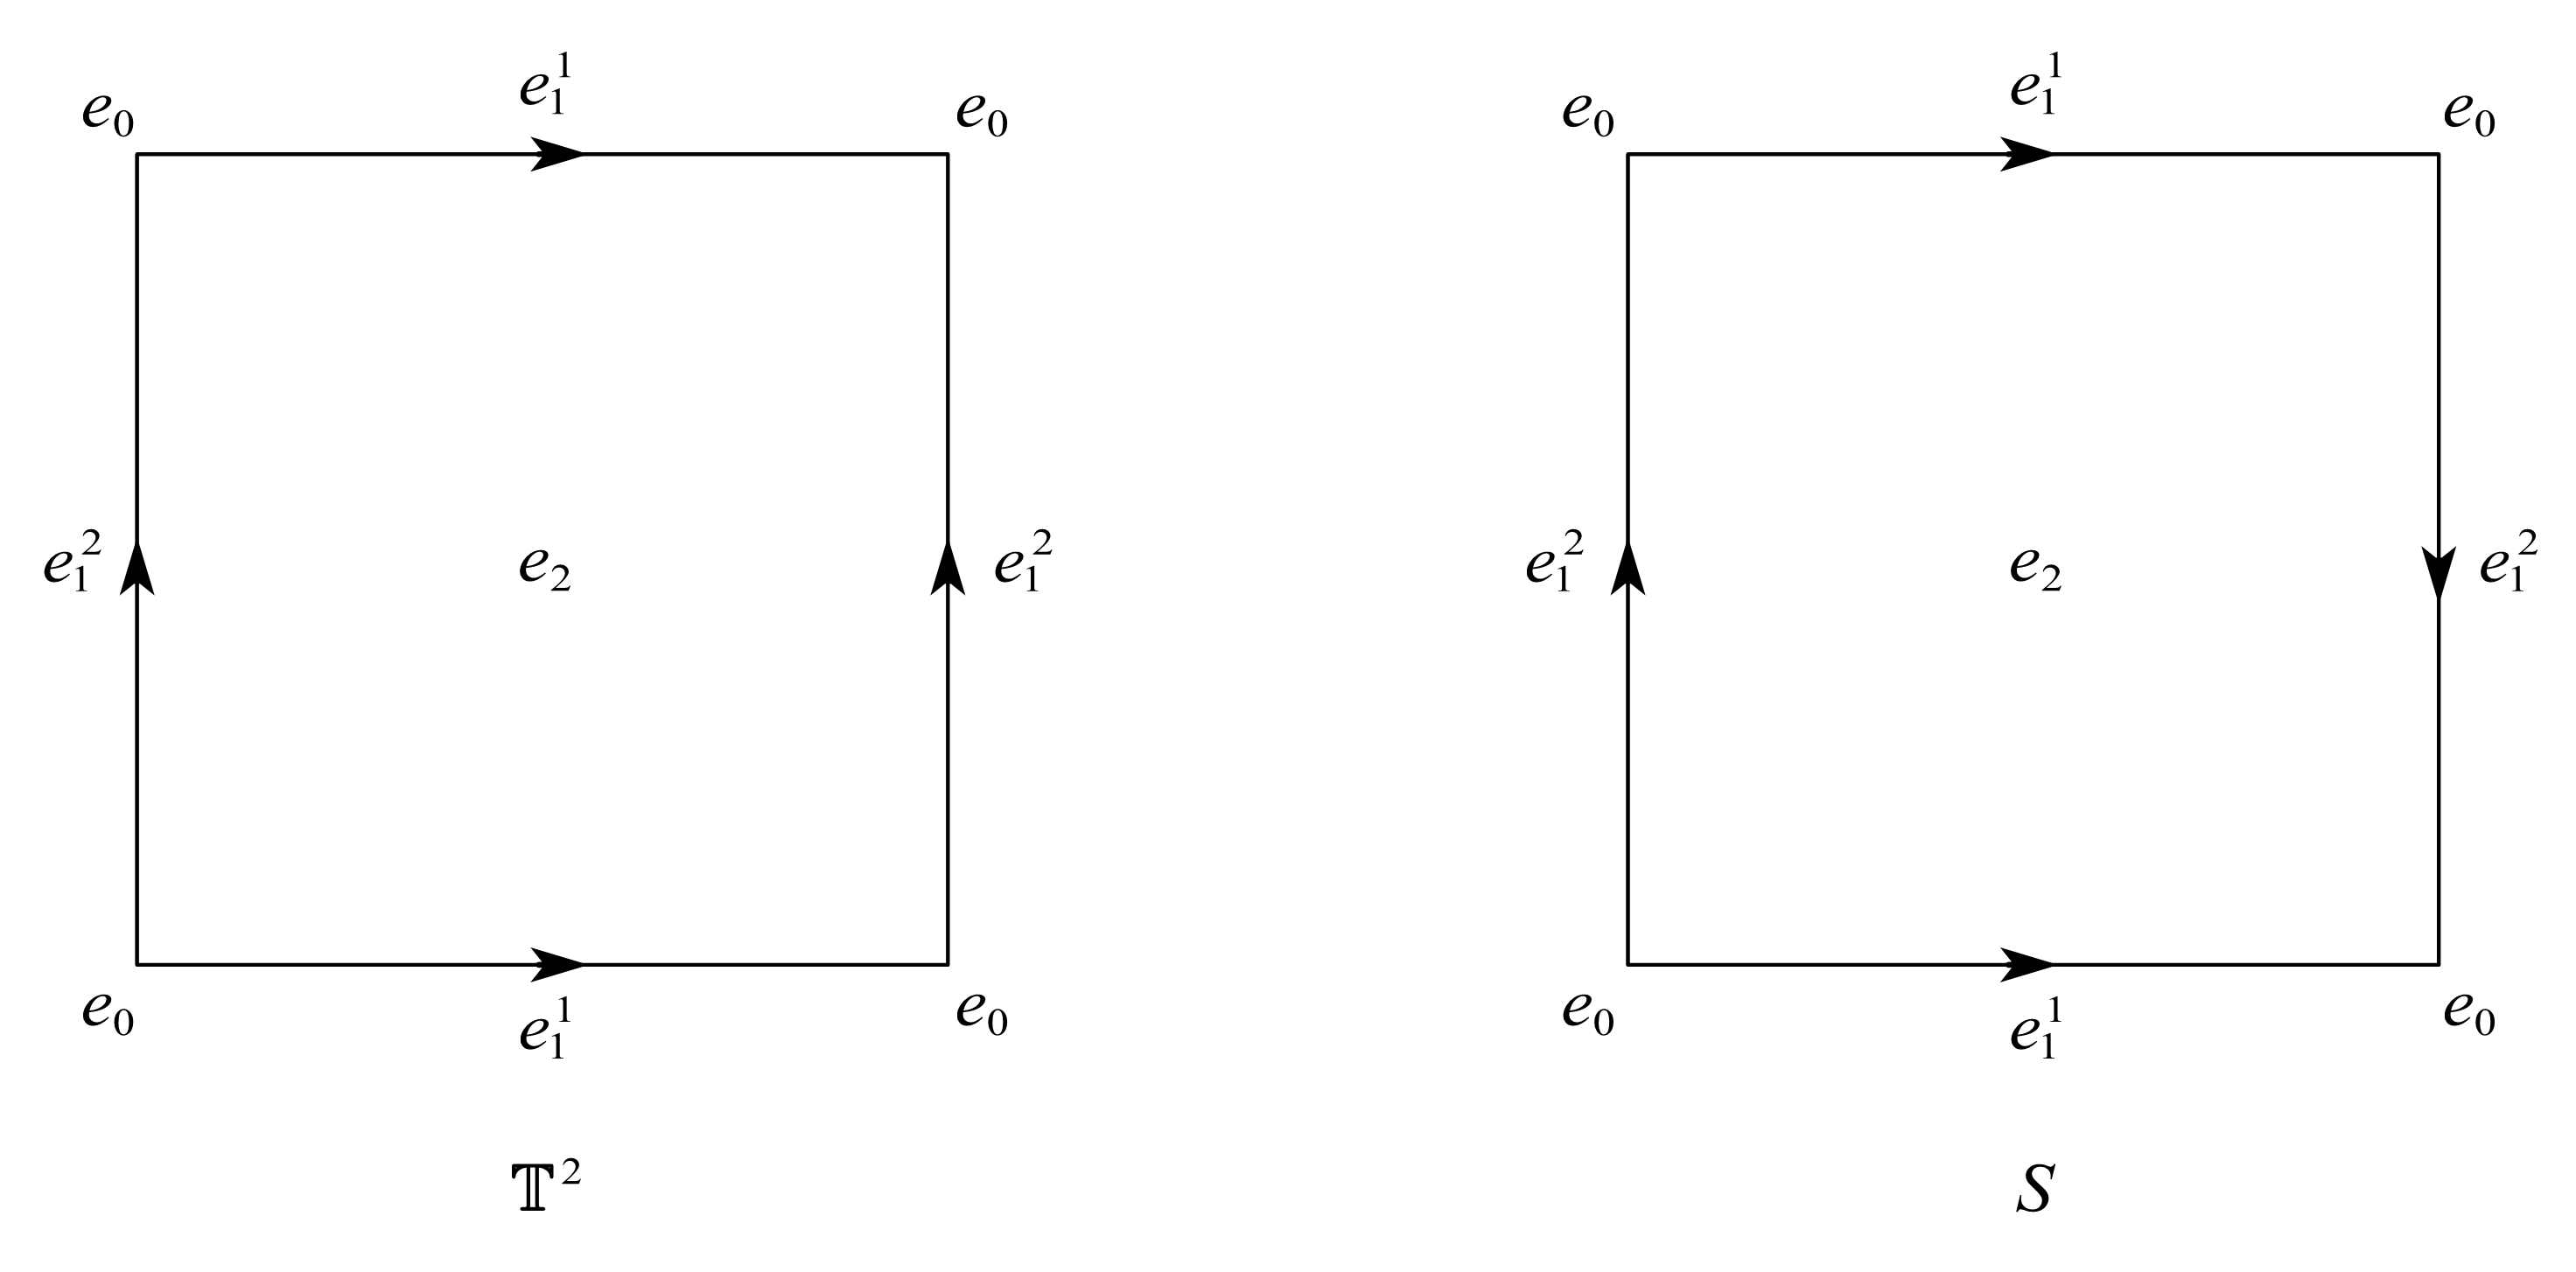
\includegraphics[width=0.4\linewidth]{figures/Sec12-1.png}
	\end{figure}
\end{Example}

\begin{Definition}[CW 复形]
	称 $ X $ 是一个 \emph{CW 复形}, 若 $ X $ 是一个拓扑空间, 一族不交的开胞腔 $ \set{e_\alpha}_{\alpha\in\CA} $ 使得 $ X=\bigcup_{\alpha\in\CA}e_\alpha $, 满足
	\begin{enumerate}
		\item $ X $ 是 Hausdorff 空间;
		\item 对任何 $ m $--开胞腔 $ e_\alpha^m $, 存在其\emph{示性映射} $ f_\alpha : \D^m\to X $ 使得 $ f_\alpha : \B^m\to e_\alpha^m $ 是一个同胚, 且 $ f_\alpha(\Bd\B^m) $ 落在有限多个维数低于 $ m $ 的开胞腔的并中; (\textit{注意这里不需要边缘与开胞腔的并相等, 只需要落在其中即可.})
		\item 对 $ A\subset X $, 若对任意 $ e_\alpha $ 都有 $ A\cap \bar{e}_\alpha $ 是 $ \bar{e}_\alpha $ 中的闭子集, 则 $ A $ 是 $ X $ 中的闭子集.(\textit{称作是 $ X $ 上的弱拓扑}).
	\end{enumerate}
	特别地, 若 $ \abs{\CA}<\infty $, 称 $ X $ 是一个\emph{有限 CW 复形}, 其\emph{维数}可由 $ \dim X=\max_{\alpha}\dim e_\alpha $ 定义. 此时 $ X $ 是 $ T_4 $ 空间.
\end{Definition}

CW 复形中, C 意为 clousre--finite, 闭有限性, 而 W 意为 weak topology, 即 (3) 中定义的拓扑.

\begin{Proposition}
	设 $ X $ 是一个 CW 复形, $ e_\alpha $ 是其一个胞腔, $ f_\alpha $ 是 $ e_\alpha $ 的示性映射. 有 $ f_\alpha(\D^m)=\bar{e}_\alpha $ 且 $ f_\alpha(\Bd\B^m)=\partial\bar{e}_\alpha $.
\end{Proposition}
\begin{Proof}
	由 $ f_\alpha $ 的连续性可知
	\[
		f_\alpha(\D^m)=f_\alpha(\bar{\B}^m)\subset\baro{f_\alpha(\B^m)}=\bar{e}_\alpha.
	\]
	反之, 因 $ \D^m $ 是紧的, 于是 $ f_\alpha(\D^m) $ 是 $ X $ 中的紧集. 因 $ X $ 是 $ T_3 $ 的, 有 $ f_\alpha(\D^m) $ 是闭集, 因此 $ \bar{e}_\alpha\subset f_\alpha(\D^m) $. 这就说明了 $ f_\alpha(\D^m)=\bar{e}_\alpha $.

	而
	\[
		\emptyset=f_\alpha(\B^m)\cap f_\alpha(\Bd\B^m)=e_\alpha\cap f_\alpha(\Bd\B^m),
	\]
	于是
	\[
		f_\alpha(\Bd\B^m)=\bar{e}_\alpha\sm e_\alpha=\partial e_\alpha.
	\]
	命题得证.\qed
\end{Proof}

\begin{Proposition}
	设 $ X $ 是 CW 复形, 那么 $ f : X\to Y $ 连续当且仅当 $ f $ 限制到每一个开胞腔 $ f|_{e_\alpha} $ 都连续.
\end{Proposition}
\begin{Proof}
	必要性是显然的, 下面证明充分性. 任取 $ B\subset Y $ 是一个闭集, 对任意的 $ e_\alpha\subset X $, 因
	\[
		f^{-1}(B)\cap e_{\alpha}=(f|_{e_\alpha})^{-1}(B)
	\]
	是 $ \bar{e}_\alpha $ 中的闭子集, 于是 $ f^{-1}(B) $ 是闭集.\qed
\end{Proof}

为了处理 CW 复形的同伦, 我们把上面的命题简单推广一下, 对 $ X $ 做一次加厚:

\begin{Corollary}
	设 $ X $ 是 CW 复形, 那么 $ f : X\times I\to Y $ 连续当且仅当对 $ X $ 的每一个开胞腔 $ e_\alpha $, $ f|_{e_\alpha\times I} $ 是连续的.
\end{Corollary}

\begin{De-Pr}[CW 子复形]\label{prop:CW 子复形}
	设 $ X $ 是一个 CW 复形, $ Y\subset X $ 是一族 $ X $ 中开胞腔的并, 且满足若 $ e_\alpha\subset Y $, 则 $ \bar{e}_\alpha\subset Y $. 则 $ Y $ 也是一个 CW 复形, 称作是 $ X $ 的 \emph{CW 子复形}. 它是 $ X $ 的闭集.
\end{De-Pr}
\begin{Proof}
	首先 $ Y $ 作为 $ X $ 的子空间是 Hausdorff 的, 且对于任意 $ e_\alpha\subset Y\susbet X $, 因 $ X $ 是 CW 复形, 存在其示性映射 $ f_\alpha : \D^m\to X $ 使得 $ f_\alpha(\D^m)=\bar{e}_\alpha\subset Y $, 于是
	\[
		f_\alpha(\Bd\B^m)\cap\set{e_\beta}_{\beta\in I_\alpha}\subset Y,
	\]
	这里 $ I_\alpha $ 是那些与 $ \bar{e}_\alpha $ 有非空交的 $ \beta $ 全体. 那么 $ f_\alpha(\Bd\B^m) $ 落在 $ Y $ 中有限多个开胞腔的并中. 这说明了闭有限性.

	设 $ B\subset Y $ 使得对任意 $ e_\alpha\subset Y $ 都有 $ B\cap\bar{e}_\alpha $ 在 $ \bar{e}_\alpha $ 中闭, 我们需要证明它在 $ Y $ 中也是闭集. 设 $ e_\beta\subset X $ 但 $ e_\beta\not\subset Y $, 则 $ e_\beta\cap Y=\emptyset $, 进而 $ \bar{e}_\beta\cap Y=\partial e_\beta $. 由定义可知 $ \bar{e}_\beta\cap Y $ 落在有限多个 $ Y $ 的开胞腔之并中, 不妨设
	\[
		\bar{e}_\beta\cap Y\subset e_{i_1}\cup\dots\cup e_{i_k},
	\]
	那么
	\[
		B\cap\bar{e}_\beta=((B\cap\bar{e}_{i_1})\cup\dots\cup(B\cap\bar{e}_{i_k}))\cap\bar{e}_\beta.
	\]
	于是 $ B\cap\bar{e}_\beta $ 在 $ \bar{e}_\beta $ 中是闭集(\textit{因后面的每一个 $ B\cap\bar{e}_{i_j} $ 都是闭的}), 于是 $ B $ 是 $ X $ 中的闭子集. 从而 $ B\cap Y=B $ 在 $ Y $ 中是闭子集. 由定义可知 $ Y $ 是
\end{Proof}

\begin{Corollary}[骨架]
	记使得 $ \dim e_\alpha=p $ 的 $ \alpha $ 全体为 $ \CA_p $, 再记 $ \CA_{\leqslant p}=\bigcup_{k\leqslant p}\CA_k $. 那么由~\ref{prop:CW 子复形}~可知
	\[
		X^p:=\bigcup_{\alpha\in\CA_{\leqslant p}}e_\alpha
	\]
	是 $ X $ 的一个 CW 子复形, 满足 $ \dim X^p=p $, 称作是 $ X $ 的 $ p $ \emph{维骨架}.
\end{Corollary}

借助骨架的概念, CW 复形可以如此归纳地定义: 在此之前先定义拓扑空间的拓扑和:

\begin{Definition}[拓扑和]
	给定两个拓扑空间 $ (X_1,\tau_1) $, $ (X_2,\tau_2) $, 在它们的无交并 $ X_1\sqcup X_2 $ 上定义拓扑
	\[
		\tau=\set{U\subset X_1\sqcup X_2 : U\cap X_i\in\tau_i},
	\]
	称如此构成的拓扑空间 $ (X_1\sqcup X_2,\tau) $ 是 $ X_1 $ 和 $ X_2 $ 的\emph{拓扑和}.
\end{Definition}

\begin{Definition}[正则 CW 复形]
	若在 CW 复形的定义中, 对每一个开胞腔 $ e_\alpha $, $ \partial e_\alpha $ 都恰是有限多个维数更低的开胞腔之并, 则称 $ X $ 是一个\emph{正则 CW 复形}.
\end{Definition}

\begin{Example}
	设 $ K $ 是一个单纯复形, 那么 $ \abs{K}=\bigcup_{\sigma\in K}\mathrm{Int}\,\sigma $ 是一个 CW 复形, 其开胞腔即为 $ \set{\mathrm{Int}\,\sigma}_{\sigma\in K} $. 特别地, 它还是一个正则 CW 复形. 设另有 $ \abs{L}=\bigcup_{\tau\in L}\mathrm{Int}\,\tau $ 也是 CW 复形, 则
	\[
		\abs{K}\times\abs{L}=\bigcup_{\sigma\in K}\bigcup_{\tau\in L}(\mathrm{Int}\,\sigma\times\mathrm{Int}\,\tau)=\bigcup_{\sigma\in K}\bigcup_{\tau\in L}\mathrm{Int}\,(\sigma\times\tau)
	\]
	仍是一个 CW 复形, 且它是一个正则 CW 复形.
\end{Example}

单纯复形对应的空间总是可以三角剖分的, 我们自然地可以去考虑 CW 复形的三角剖分. 仍然希望一些比较好的 CW 复形可以和单纯复形扯上那么一点儿关系.

\begin{Definition}[三角剖分]
	称 $ K $ 是一个\emph{可三角剖分}的 CW 复形, 若存在同胚 $ h : X\to\abs{K} $ 满足对任意 $ p\in\Z $, 存在 $ K $ 的子复形 $ L $, $ \dim L\leqslant p $ 使得 $ h|_{X^p} : X^p\to \abs{L} $ 是同胚.
\end{Definition}

需要注意的是, 单纯复形与 CW 复形本身是有一些区别的. 对 $ n $ 维单纯复形 $ K $, 总有
\[
	K^{(0)}\subsetneqq K^{(1)}\subsetneqq\dots\subsetneqq K^{(n)}=K,
\]
其中的每一项与前一项的差都是非零的, 每一个包含关系都是严格的. 但对 $ n $ 维 CW 复形 $ X $, 上述关系变成
\[
	X^0\subset X^1\subset\dots\subset X^n=X,
\]
只有 $ X^0 $ 一定非零, $ X^n $ 与前一项的差一定非零, 中间的包含关系都有可能相等. 例如对 CW 复形 $ \S^n $ 就有 $ X^0=X^1=\dots=X^{n-1} $.

\begin{Example}
	对球面 $ X=\S^n $, 它有三角剖分 $ h : X\to\abs{K} $ 使得对任何的 $ p\leqslant n-1 $, 都有 $ h|_{X^{p}} : X^p\to\abs{K}^{(0)} $, 这因 $ X^0=X^1=\dots=X^{n-1} $, 而 $ h : X\to\abs{K} $.
	\begin{figure}[htbp]
		\centering
		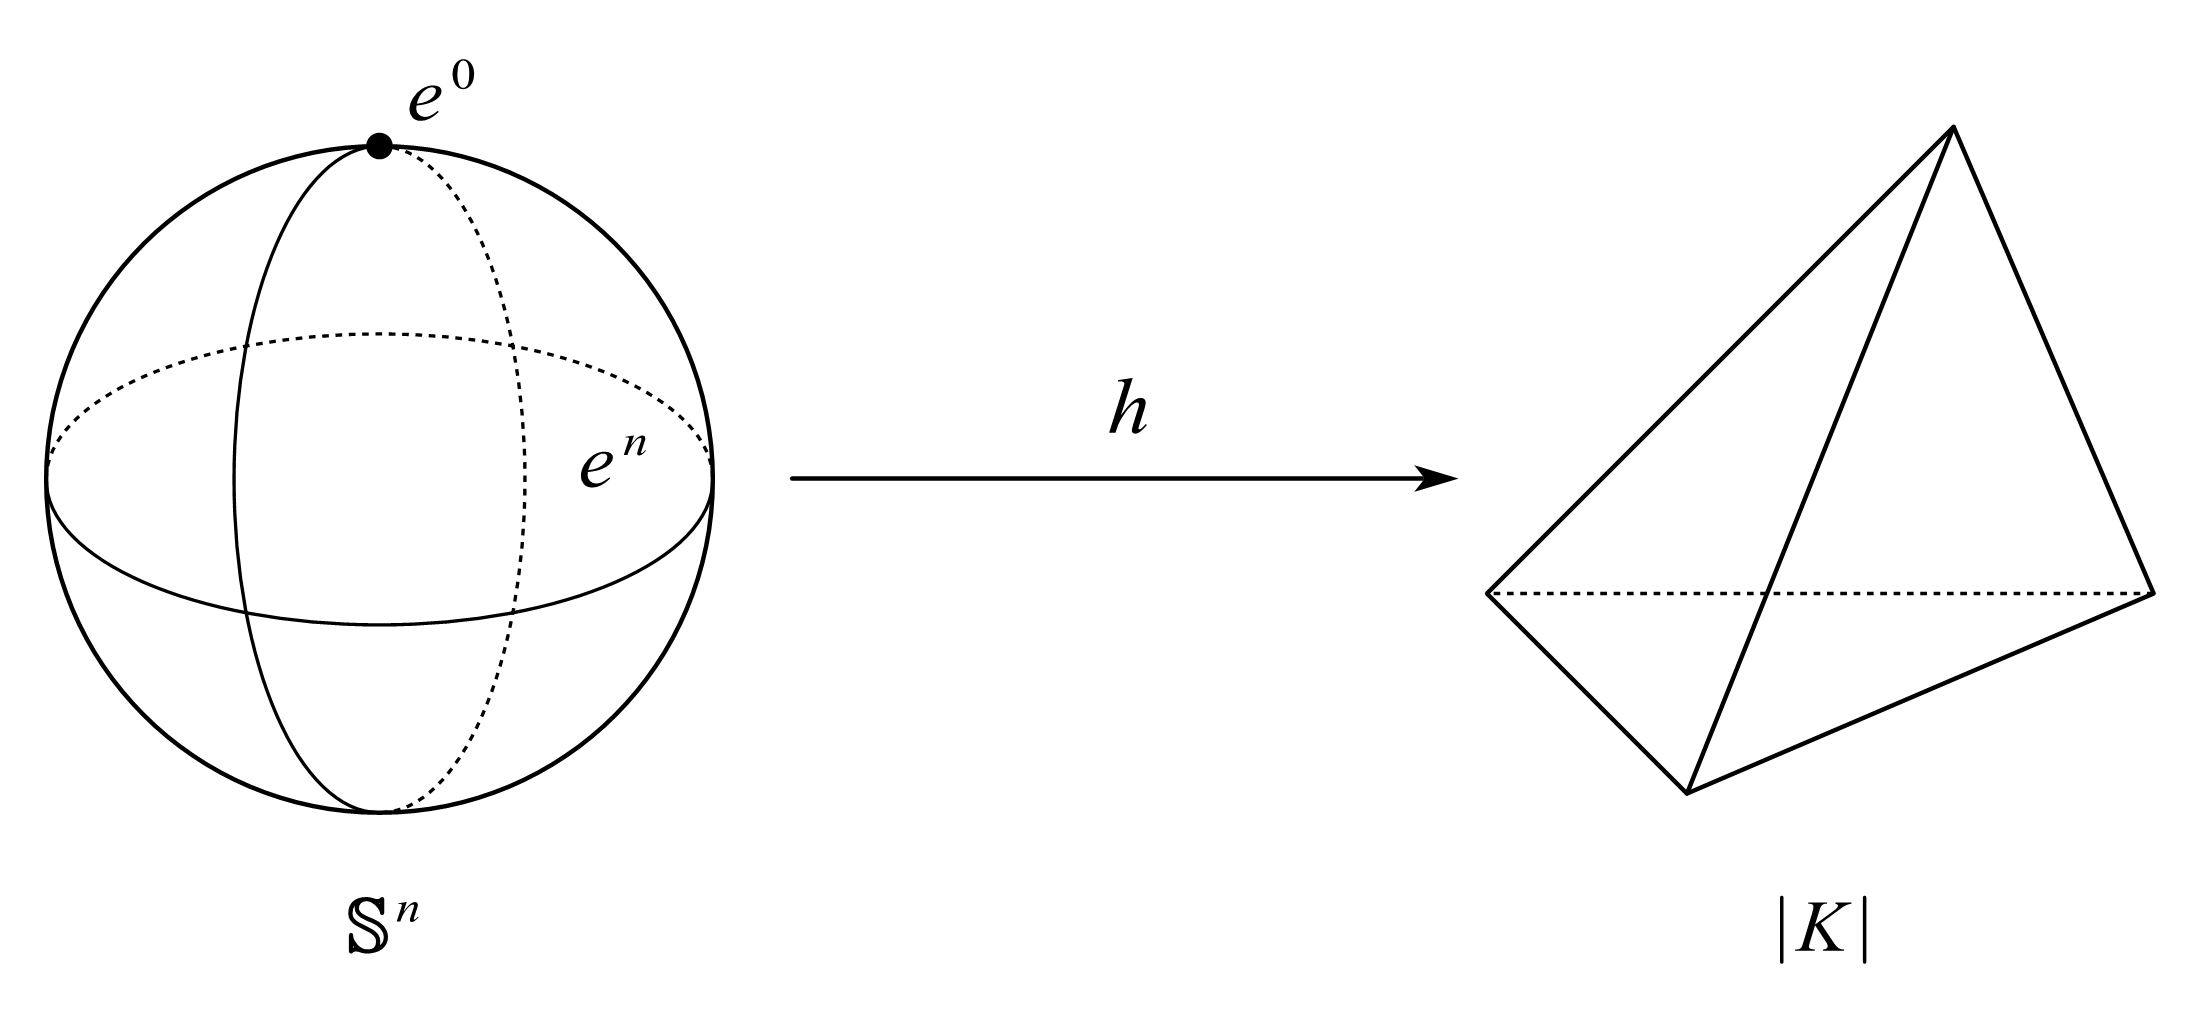
\includegraphics[width=0.55\linewidth]{figures/Sec12-2.png}
	\end{figure}
\end{Example}

\begin{Example}[不可三角剖分的 CW 复形]
	下面构造一个不可三角剖分的 CW 复形, 考虑一个正方形粘上一个三角形构成的单纯复形 $ K $, 其几何实现记作 $ A $. 在正方形上存在一条曲线 $ (x,\sin 1/x) $, 记作 $ C $, 那么 $ \bar{C}\subset A $. 将正方形与三角形相交的线记作 $ D $, 并如此定义 CW 复形:
	\begin{figure}[htbp]
		\centering
		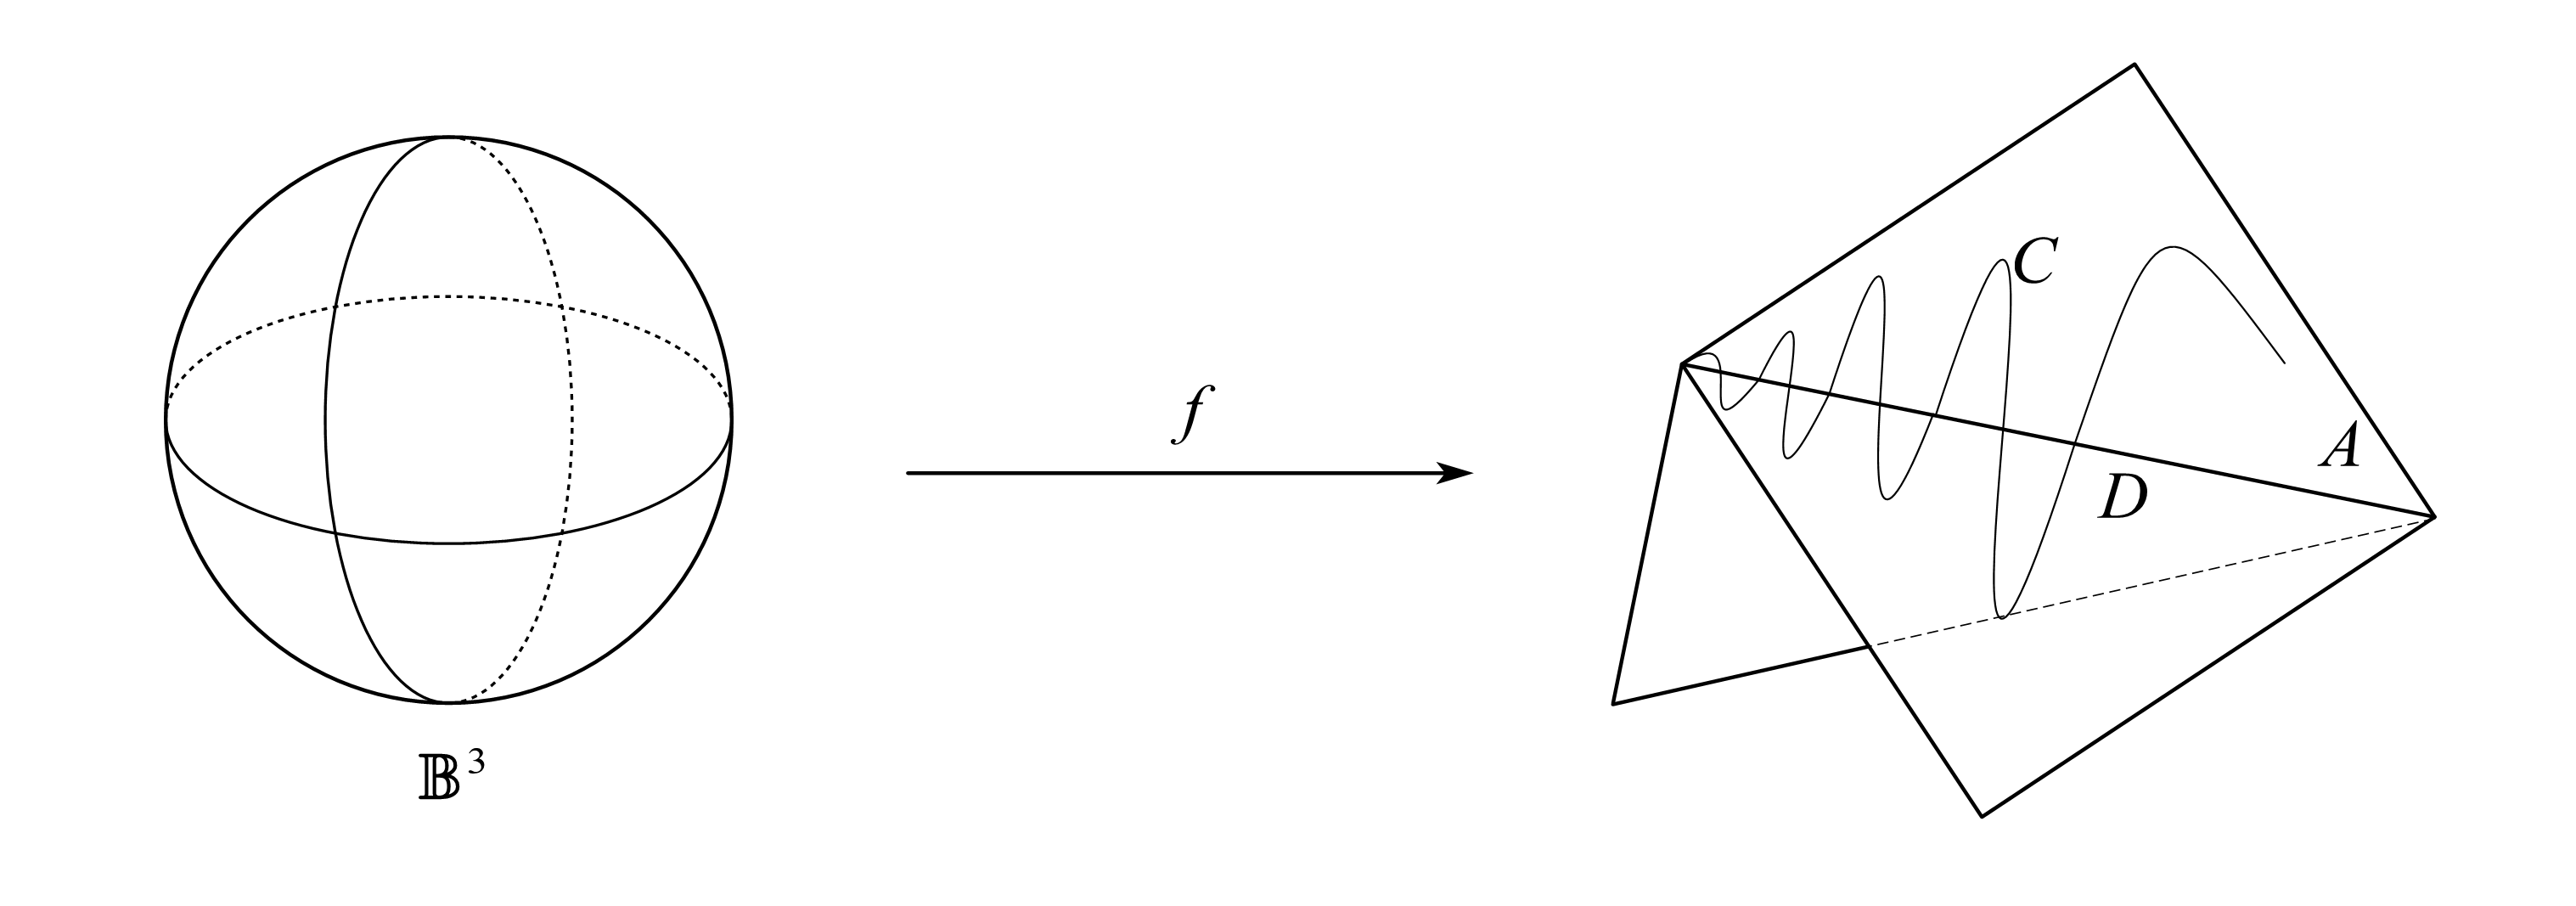
\includegraphics[width=0.65\linewidth]{figures/Sec12-3.png}
	\end{figure}\\
	黏合映射 $ g : \Bd\B^3\to\bar{C}\subset A $, 此时 $ X=A\sqcup_g\B^3 $ 具有 CW 复形结构, 并且映射
	\[
		\pi : A\sqcup\B^3\to A\sqcup_g\B^3
	\]
	满足 $ \pi|_{\Bd\B^3}=g $, 于是 $ \pi(\mathrm{Int}\,\B^3)=e_3 $ 就是三角形内部构成的胞腔.

	由此确定的 $ X $ 是不可三角剖分的, 为了证明这一断言, 我们使用反证法. 否则, 存在单纯复形 $ L $ 使得
	\[
		h : \abs{L}\to X=(A\sm C)\cup C\cup e_3
	\]
	是一个同胚.

	首先考虑 $ \bar{e}_3 $, 取 $ x\in e_3 $ 有
	\[
		H_3(X,X\sm x)\cong H_3(\B^3,\B^3\sm 0)\cong H_3(\B^3,\S^2)\cong\Z.
	\]
	取 $ x\in A\sm C $ 有
	\[
		H_3(X,X\sm X)\cong H_3(\B^2,\B^2\sm 0)=0
	\]
	中间的一项也可能是 $ H_3(\B_+^2,\B_+^2\sm 0) $, 这源于切除公理中取 $ U=X\sm\B^2 $ 或是 $ U=X\sm \B_+^2 $, 取决于 $ x $ 位于内部还是边界. 而对 $ \sigma\in L $, $ h(\mathrm{Int}\,\sigma) $ 不可能同时与 $ e_3 $ 和 $ A\sm C $ 相交. 这因对任何 $ x,y\in\mathrm{Int}\,\sigma\subset\abs{K} $, 都有
	\[
		H_p(\abs{K},\abs{K}\sm x)\cong H_p(\abs{K},\abs{K}\sm y).
	\]
	于是 $ h(\mathrm{Int}\,\sigma) $ 或者是属于 $ \bar{e}_3 $ 的, 或者是属于 $ A=\baro{A\sm C} $ 的. 由此, $ \bar{e}_3 $ 和 $ A $ 都分别可以三角剖分.

	同样地, 断言 $ D $ 也可以被 $ h $ 三角剖分. 因 $ D\subset A $, 取 $ x\in\mathrm{Int}\,D $. 注意到 $ A=x*\partial A $ 可缩, 由长正合序列可得
	\[
		H_2(A,A\sm x)\cong H_1(A\sm x)\cong\Z\oplus\Z,
	\]
	这因此时 $ A\sm x $ 实际上同伦于 8 字形空间. 取 $ x\in A\sm D $, 就有
	\[
		H_2(A,A\sm x)\cong\begin{cases}
			H_2(\B_+^2,\B_+^2\sm 0), &x\in\partial A\sm D\\ H_2(\B^2,\B^2\sm 0), &x\notin \partial A
		\end{cases}
	\]
	于是对任意 $ \sigma\in L $, 也有 $ h(\mathrm{Int}\,\sigma)\cap D=\emptyset $, 那么 $ h(\sigma)\subset D $, 于是 $ D $ 也可以被 $ h $ 三角剖分.

	进而 $ \bar{C}\cap D $ 也可被 $ h $ 三角剖分. 但这不可能成立, 因为 $ \bar{C} $ 与 $ D $ 相交于无穷多个点.
\end{Example}

直观上讲, 从一个离散点集 $ X^0 $ 开始, 在 $ X^0 $ 上定义离散拓扑. 按照如下的方式从 $ X^{p-1} $ 构造 $ X^p $: 将 $ \D^p $ 通过黏合映射 $ \varphi : \Bd\D^p\to X^{p-1} $ 粘到 $ X^{p-1} $ 上, 那么在拓扑和 $ X^{p-1}\sqcup\D^p $ 上定义等价关系:
\[
	\forall x\in\Bd\D^p\,(x\sim\varphi(x)),
\]
从而 $ X^p=X^{p-1}\sqcup\D^p/\sim $.

\subsection{CW 复形的结构}

\begin{Theorem}
	设 $ X $ 是 $ p $ 维的 CW 复形, 则
	\begin{enumerate}
		\item $ X=X^{p-1}\sqcup_g(\sum\D_\alpha^p) $, 这里 $ \sum $ 表示拓扑和, $ g : \sum\Bd\D_\alpha^p\to X^p $.
		\item 设 $ Y $ 是一个 CW 复形, $ \dim Y\leqslant p-1 $, $ g : \sum\Bd\D_\alpha^p\to Y $ 使得 $ g $ 将每一个 $ \Bd\D_\alpha^p $ 映到有限多个 $ Y $ 的开胞腔中. 那么 $ X=Y\sqcup_g(\sum\D_\alpha^p) $ 是一个 CW 复形, 且 $ Y=X^{p-1} $.
	\end{enumerate}
\end{Theorem}
\begin{Proof}
	(1) 设 $ e_\alpha\subset X $ 是一个 $ p $--开胞腔, 其示性映射 $ f_\alpha : \D_\alpha^p\to\bar{e}_\alpha\subset X $. 令 $ \D_\alpha^p=\D^p\times\set{\alpha} $, 做拓扑和
	\[
		E=X^{p-1}\sqcup(\Sigma\D_\alpha^p).
	\]
	取 $ g : \sum\Bd\D_\alpha^p\to X^p $ 满足 $ g|_{\Bd\D_\alpha^p}=f_\alpha|_{\Bd\D_\alpha^p} $. 考虑映射
	\[
		\pi : E=X^{p-1}\sqcup(\Sigma\D_\alpha^p)\to X^{p-1}\sqcup_g(\Sigma\D_\alpha^p),
	\]
	它满足 $ \pi|_{X^{p-1}}=\iota : X^p\hookrightarrow X $, $ \pi|_{\sum\Bd\D_\alpha^p}=g $, $ \pi|_{\sum\mathrm{Int}\,D_\alpha^p}=\sum f_\alpha |_{\sum\mathrm{Int}\,\D_\alpha^p} $. 只需要证明 $ \pi $ 是商映射即可, 进而只需证它是闭映射, 也即 $ C\subset X $ 是闭集当且仅当 $ \pi^{-1}(C) $ 是闭集.

	必要性是显然的, 因 $ \pi $ 是连续的. 下设 $ \pi^{-1}(C) $ 是闭集, 因
	\[
		\pi^{-1}(C)\cap X^{p-1}=C\cap X^{p-1}
	\]
	是 $ X^{p-1} $ 中的闭集, 于是对任意 $ e_\beta\subset X^{p-1} $, 有
	\[
		C\cap\bar{e}_\beta=(C\cap X^{p-1})\cap\bar{e}_\beta
	\]
	是 $ \bar{e}_\beta $ 中的闭集. 再考虑 $ \pi^{-1}(C)\cap\D_\alpha^p $ 是 $ \D_\alpha^p $ 中的闭集, 故对任何满足 $ \dim e_\alpha=p $ 的开胞腔 $ e_\alpha\subset X $, 因
	\[
		C\cap\bar{e}_\alpha=\pi(\pi^{-1}(C)\cap\D_\alpha^p)
	\]
	是 $ X $ 中的紧子集(\textit{因 $ \pi $ 连续而后者是 $ T_4 $ 空间上紧集的闭子集, 从而仍是紧的}), 从而是 $ X $ 中的闭集. 因 $ X $ 是 Hausdorff 的, 于是 $ C\cap\bar{e}_\alpha $ 在 $ \bar{e}_\alpha $ 中也是闭集, 那么弱拓扑导出 $ C $ 是闭集.

	(2) 有投射
	\[
		\pi : Y\sqcup(\Sigma\D_\alpha^p)\to X=Y\sqcup_g(\Sigma\D_\alpha^p),
	\]
	同样只需 $ \pi $ 是商映射, 同样只需证它是闭映射. 必要性仍然是显然的, 因 $ \pi $ 是连续的. 下设 $ \pi^{-1}(C) $ 是闭集, 因为 $ Y\sqcup(\sum\D_\alpha^p) $ 是 $ T_4 $ 的, 故 $ \pi^{-1}(C) $ 是紧的. 因为 $ \pi $ 连续, $ \pi(\pi^{-1}(C)) $ 在 $ X $ 中是紧的, 从而是闭的.
	
	那么 $ X $ 的胞腔只有两种: 其一是 $ Y $ 中 $ \dim\leqslant p-1 $ 的开胞腔, 另一种是 $ p $--开胞腔, 它们有 $ \pi(\mathrm{Int}\,\D_\alpha^p)=e_\alpha $ 粘合而来. 因为
	\[
		\pi^{-1}(\pi(\mathrm{Int}\,\D_\alpha^p))=\mathrm{Int}\,\D_\alpha^p\subset\D_\alpha^p
	\]
	是开集, 于是 $ \pi|_{\mathrm{Int}\,\D_\alpha^p} : \mathrm{Int}\,\D_\alpha^p\to\pi(\mathrm{Int}\,D_\alpha^p) $ 是一个同胚, 此时 $ \pi|_{\D_\alpha^p}=:f_\alpha $ 就是 $ e_\alpha $ 的示性映射. 因此 $ X $ 的确是一族不交开胞腔的并, 下面逐条验证它满足 CW 复形的定义:

	(2a) $ X $ 是 $ T_4 $ 的, 于是必然是 Hausdorff 的.

	(2b) 对任意 $ e_\beta\subset Y $, 因为 $ Y $ 是 CW 复形, 那么在 $ Y $ 上存在示性映射 $ f_\beta : \D_\beta\to\bar{e}_\beta\subset Y\subset X $, 将其复合上一个嵌入映射就得到它在 $ X $ 上的示性映射. 而对于 $ e_\alpha\subset X\sm Y $, 由前述讨论可知它的示性映射 $ f_\alpha $ 即为 $ \pi|_{\D_\alpha^p} $, 特别地, $ f_\alpha|_{\Bd\D_\alpha^p}=g|_{\Bd\D_\alpha^p} $ 满足有限性.

	(2c) 对 $ C\subset X $, 若对任何 $ e_\alpha\subset X $ 都有 $ C\cap\bar{e}_\alpha $ 是 $ \bar{e}_\alpha $ 中的闭集, 只需要 $ \pi^{-1}(C) $ 也是闭集即可. 而这由
	\[
		\pi^{-1}(C)=\pi^{-1}(C)\cap(Y\cup(\Sigma\D_\alpha^p))=(\pi^{-1}(C)\cap Y)\cup(\Sigma(\pi^{-1}(C)\cap\D_\alpha^p)).
	\]
	因 $ Y $ 是 CW 复形, $ \pi $ 限制到 $ Y $ 上是嵌入, 于是 $ \pi^{-1}(C)\cap Y=C\cap Y $ 借助在 $ Y $ 上的弱拓扑是闭集. 而对后一项, 注意到
	\[
		\pi^{-1}(C)\cap\D_\alpha^p=\pi^{-1}(C\cap\bar{e}_\alpha)\cap\D_\alpha^p
	\]
	因 $ C\cap\bar{e}_\alpha $ 是闭的, 故 $ \pi^{-1}(C\cap\bar{e}_\alpha) $ 作为连续映射的原像是闭的, 而 $ D_\alpha^p $ 是闭集, 从而 $ \pi^{-1}(C)\cap\D_\alpha^p $ 也是闭集. 这就说明了 $ X $ 上具有弱拓扑.
	
	而此时新添加进来的胞腔都是 $ p $ 维的, 于是 $ Y=X^{p-1} $.\qed
\end{Proof}

\subsection{胞腔链复形}

对 CW 复形 $ X $, 其奇异链复形自然可以诱导出同调群, 但经过之前对于奇异同调的讨论不难发现, 奇异同调的确难以计算. 于是借助 CW 复形上的胞腔结构, 我们可以类似单纯链复形定义胞腔链复形. 在直观上, 胞腔链复形中的 $ p $ 维链群就是由 $ X $ 的 $ p $--开胞腔生成的自由 Abel 群.

\begin{Definition}[胞腔链复形]
	设 $ X $ 是 CW 复形, 有 $ X^0\subset X^1\subset\dots\subset X^p\susbet\cdots $, 这是一列极限是 $ X $ 的空间. 取
	\[
		D_p(X)=H_p(X^p,X^{p-1}),
	\]
	称作是 $ X $ 的 $ p $ \emph{维胞腔链群}. 边缘运算 $ \partial : D_p(X)\to D_{p-1}(X) $ 通过以下的正合序列
	\begin{center}
		\begin{tikzcd}
			&                                                                   & {} \arrow[d]                                &                        &    \\
			&                                                                   & H_{p-1}(X^{p-2}) \arrow[d]                  &                        &    \\
{} \arrow[r] & {H_p(X^p,X^{p-1})} \arrow[r, "\partial_*"] \arrow[rd, "\partial"] & H_{p-1}(X^{p-1}) \arrow[r] \arrow[d, "j_*"] & H_{p-1}(X^p) \arrow[r] & {} \\
			&                                                                   & {H_{p-1}(X^{p-1},X^{p-2})} \arrow[d]        &                        &    \\
			&                                                                   & {}                                          &                        &   
		\end{tikzcd}
	\end{center}
	中的 $ \partial=j_*\partial_* $ 确定. 称 $ \CD(X):=\set{(D_p(X),\partial)} $ 是 $ X $ 的\emph{胞腔链复形}.
\end{Definition}

\begin{Proposition}
	$ \partial^2=0 $.
\end{Proposition}
\begin{Proof}
	这因
	\begin{center}
		\begin{tikzcd}
			  & {H_p(X^p,X^{p-1})} \arrow[d, "\partial_*"] \arrow[rd, "\partial_p"] &                                                                                  &                                              &      \\
{} \arrow[r] & H_{p-1}(X^{p-1}) \arrow[r, "j_*"]                                   & {H_{p-1}(X^{p-1},X^{p-2})} \arrow[r, "\partial'_*"] \arrow[rd, "\partial_{p-1}"] & H_{p-2}(X^{p-2}) \arrow[r] \arrow[d, "j'_*"] & {} \\
                         &                                                                     &                                                                                  & {H_{p-2}(X^{p-2},X^{p-3})}                   &                           
		\end{tikzcd}
	\end{center}
	注意到中间的一行是正合列即可.\qed
\end{Proof}

关于 $ \partial : D_p(X)\to D_{p-1}(X) $ 的定义, 还可以从另一个角度来看待. 考虑三元组 $ (X^p,X^{p-1},X^{p-2}) $ 确定的正合列
\begin{center}
	\begin{tikzcd}
		0 \arrow[r] & {\CS(X^{p-1},X^{p-2})} \arrow[r, hook] & {\CS(X^p,X^{p-2})} \arrow[r, two heads] & {\CS(X^p,X^{p-1})} \arrow[r] & 0
	\end{tikzcd}
\end{center}
由 zig--zag 引理, 它诱导长正合列
\begin{center}
	\begin{tikzcd}
		\cdots \arrow[r] & {H_p(X^{p-1},X^{p-2})} \arrow[r] & {H_p(X^p,X^{p-2})} \arrow[r] & {H_p(X^p,X^{p-1})} \arrow[r, "\partial_*"] \arrow[d, Rightarrow, no head] & {H_{p-1}(X^{p-1},X^{p-2})} \arrow[r] \arrow[d, Rightarrow, no head] & \cdots \\
						 &                                  &                              & D_p(X) \arrow[r, "\partial"]                                              & D_{p-1}(X)                                                          &       
	\end{tikzcd}
\end{center}
于是 $ \partial $ 就是 $ \partial_* $. (之后我们使用 $ \dot{e}_\alpha $ 来表示之前的 $ \partial e_\alpha $, 为了防止与这里定义的 $ \partial $ 混淆.)

\begin{Proposition}
	对单纯复形 $ K $, $ X=\abs{K} $ 上有自然的 CW 复形结构. 此时 $ H_p(\CD(K))\cong H_p(\CS(K))\cong H_p(\CC(K)) $.
\end{Proposition}
\begin{Proof}
	因为对这样的 $ X $, 有 $ X=\abs{K} $, $ X^p=\abs{K^{(p)}} $, 那么
	\[
		D_p(X)=H_p(X^p,X^{p-1})=H_p(K^{(p)},K^{(p-1)}),
	\]
	因为
	\[
		C_i(K^{(p)},K^{(p-1)})=\begin{cases}
			0 & ,i\ne p \\ C_p(K^{(p)})=C_p(K) & ,i=p
		\end{cases}
	\]
	于是 $ \CC(K^{(p)},K^{(p-1)}) $ 只有在 $ i=p $ 处非平凡, 于是 $ D_p(K)=C_p(K) $. 这就证明了结论.\qed
\end{Proof}

我们先考虑粘上一个开胞腔的情况: 考虑 $ e_\alpha\subset X $, $ \dim e_\alpha=p $.
\begin{figure}[htbp]
	\centering
	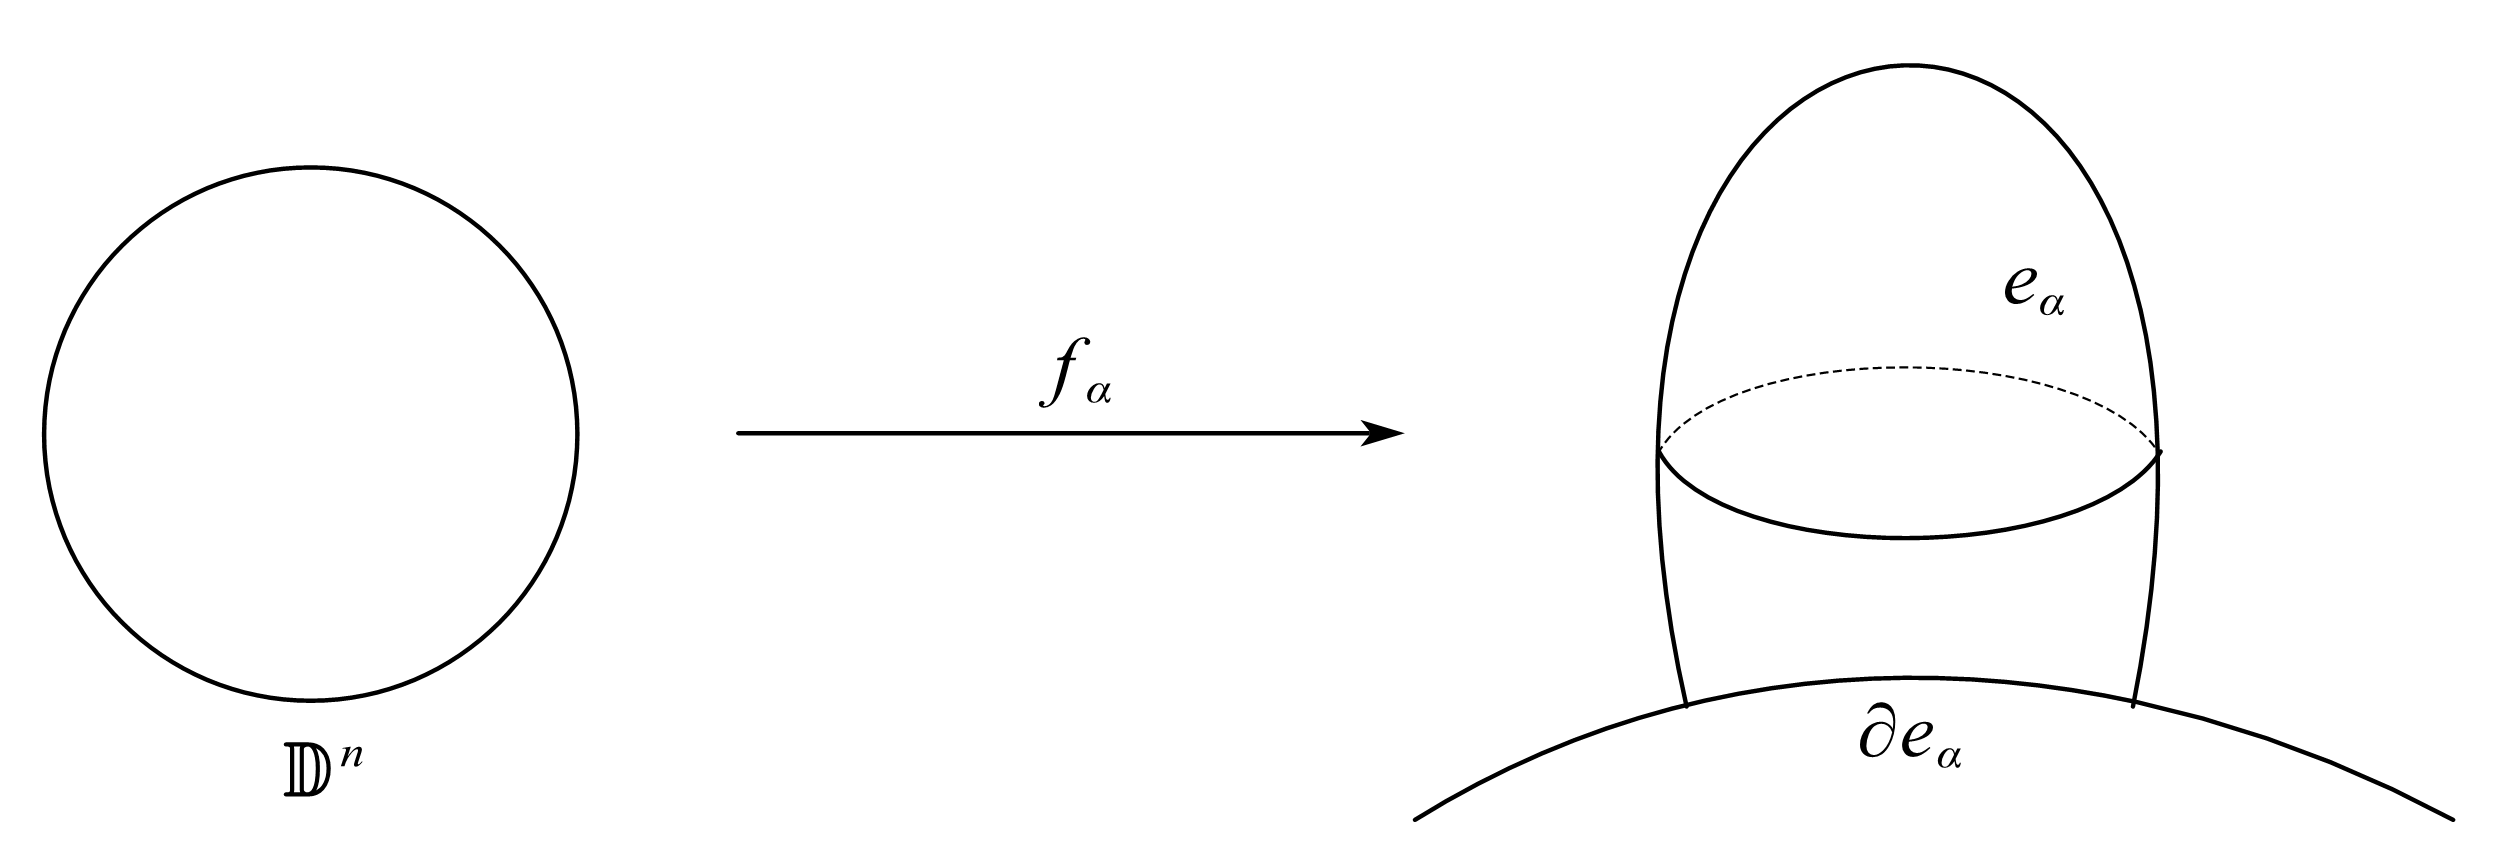
\includegraphics[width=0.5\linewidth]{figures/Sec13-1.png}
\end{figure}

\begin{Lemma}
	对 CW 复形 $ X $ 中的 $ p $--开胞腔 $ e_\alpha $, 其示性映射
	\[
		f_\alpha : (\D^p,\S^{p-1})\to(\bar{e}_\alpha,\dot{e}_\alpha)
	\]
	诱导了一个相对同调的同构.
\end{Lemma}
\begin{Proof}
	$ n=0 $ 时自然成立, 因此不妨假设 $ n>0 $. 取 $ 0\in\D^n $, 记 $ \hat{e}_\alpha=f_\alpha(0) $, 则
	\[
		f_\alpha : \D^n\sm 0\to\bar{e}_\alpha\sm\hat{e}_\alpha
	\]
	仍是商映射. $ \D^n\sm 0 $ 可以形变收缩到 $ \S^{n-1} $, 于是 $ H' $ 可以由下图诱导:
	\begin{center}
		\begin{tikzcd}
			(\D^n\sm 0)\times I \arrow[d, "H"'] \arrow[r, "f_\alpha\times\id_I"] & (\bar{e}_\alpha\sm\hat{e}_\alpha)\times I \arrow[d, "H'"] \\
			\D^n\sm 0 \arrow[r, "f_\alpha"]                                      & \bar{e}_\alpha\sm\hat{e}_\alpha                          
		\end{tikzcd}
	\end{center}
	此时有
	\begin{center}
		\begin{tikzcd}
			{(\D^n,\S^{n-1})} \arrow[d, "f_\alpha"'] \arrow[r, "\cong", hook] & {(\D^n,\D^n\sm 0)}                                 & {(\mathrm{Int}\,\D^n,\mathrm{Int}\,(\D^n\sm 0))} \arrow[l, "\cong"', hook'] \arrow[d, "f_\alpha"] \\
			{(\bar{e}_\alpha,\dot{e}_\alpha)} \arrow[r, "\cong", hook]        & {(\bar{e}_\alpha,\bar{e}_\alpha\sm\hat{e}_\alpha)} & {(e_\alpha,e_\alpha\sm\hat{e}_\alpha)} \arrow[l, "\cong"', hook']                                
		\end{tikzcd}
	\end{center}
	其中右侧的两个同胚分别取 $ U=\Bd\B^n $ 和 $ U=\dot{e}_\alpha $ 由切除公理得到.\qed
\end{Proof}

我们考虑把所有的 $ p $ 维开胞腔都粘上的情况, $ D_p(X)=H_p(X^p,X^{p-1}) $, $ \sum f_\alpha : \sum(\D^p_\alpha,\S_\alpha^{p-1})\to(X^p,X^{p-1}) $, 则对 $ X^p=X^{p-1}\sqcup_g(\sum\D_\alpha^p) $. 这时黏合映射 $ g : \sum(\Bd\D_\alpha^p)\to X^{p-1} $.

\begin{Lemma}
	$ H_i(X^p,X^{p-1})\cong H_i(\sum\D_\alpha^p,\sum\S_\alpha^{p-1})\cong\bigoplus_{\alpha\in\CA_p}H_i(\D_\alpha^p,\S_\alpha^{p-1}) $.
\end{Lemma}
\begin{Proof}
	考虑
	\[
		\pi : X^{p-1}\sqcup(\Sigma(\D_\alpha^p\sm 0))\to X^{p-1}\sqcup_g(\Sigma(\D_\alpha^p\sm 0)),
	\]
	而前者同伦于 $ X^{p-1}\sqcup(\sum\S_\alpha^{p-1}) $, 后者即为 $ \pi(X^{p-1}\sqcup(\sum\D_\alpha^p\sm 0))=X^{p-1}\sqcup(\sum\bar{e}_\alpha\sm\hat{e}_\alpha) $, 而这同伦于 $ X^{p-1} $. 类似地有
	\begin{center}
		\begin{tikzcd}
			{(\Sigma\D_\alpha^p,\Sigma\Bd\D_\alpha^p)} \arrow[d, "\pi"'] \arrow[r, "\cong", hook] & {(\Sigma\D_\alpha^p,\Sigma(\D_\alpha^p\sm 0))}  & {(\Sigma\mathrm{Int}\,\D_\alpha^p,\Sigma\mathrm{Int}\,(\D_\alpha^p\sm 0))} \arrow[l, "\cong"', hook'] \arrow[d, "{\pi=\sum f_\alpha|_{\sum\mathrm{Int}\,\D_\alpha^p}}"] \\
			{(X^p,X^{p-1})} \arrow[r, "\cong", hook]                                              & {(X^p,X^p\sm\bigcup\hat{e}_\alpha)}             & {(\bigcup e_\alpha,\bigcup(e_\alpha\sm\hat{e}_\alpha))} \arrow[l, "\cong"', hook']                                                           
		\end{tikzcd}
	\end{center}
	而最右侧的 $ \pi $ 是同胚. 于是
	\[
		H_i(X^p,X^{p-1})\cong H_i(\Sigma\B_\alpha^p,\Sigma\Bd\,\D_\alpha^p)\cong\bigoplus_\alpha H_i(\bar{e}_\alpha,\dot{e}_\alpha),
	\]
	且只有 $ i=p $ 时, 右侧是非零的. 并且 $ H_p(X^p,X^{p-1})=\Z^{\oplus\abs{\CA_p}} $.\qed
\end{Proof}

尽管链复形中的 $ D_p(X) $ 看起来非常显然, 这里 $ \abs{\CA_p} $ 就是 $ p $--开胞腔的个数, 但此时 $ \partial $ 的具体确定却成为了难点. 特别地, 若 $ X $ 是可以三角剖分的 CW 复形时, $ \partial $ 的确定相对容易一些, 这因为 $ \partial $ 和链映射的交换性可以让我们直接对单纯复形讨论边缘算子.

\subsection{胞腔同调与奇异同调的等价性}

在讨论与奇异同调的关系之前, 我们首先说明胞腔复形的所谓定向. 对 $ \alpha\in\CA_p $, 有 $ H_p(\bar{e}_\alpha,\dot{e}_\alpha)\cong\Z $, 后者有生成元 $ \pm 1 $, 于是 $ H_p(\bar{e}_\alpha,\dot{e}_\alpha) $ 的生成元就确定了 $ e_\alpha $ 的定向.

\begin{Theorem}
	设 $ X $ 是 CW 复形, 则 $ H_p(\CD(X))\cong H_p(\CS(X)) $.
\end{Theorem}
\begin{Proof}
	当 $ X=\abs{K} $ 时已经证明过了, 我们考虑一般情况. 直接计算
	\begin{center}
		\begin{tikzcd}
			{} \arrow[r] & D_{p+1}(X) \arrow[r] \arrow[d, Rightarrow, no head] & D_p(X) \arrow[r] \arrow[d, Rightarrow, no head] & D_{p-1}(X) \arrow[r] \arrow[d, Rightarrow, no head] & {} \\
						 & {H_{p+1}(X^{p+1},X^p)}                              & {H_p(X^p,X^{p-1})}                              & {H_{p-1}(X^{p-1},X^{p-2})}                          &   
		\end{tikzcd}
	\end{center}
	这涉及四个骨架 $ (X^{p+1},X^p,X^{p-1},X^{p-2}) $, 它产生了四个三元组
	\[
		(X^{p+1},X^p,X^{p-1}) ,  (X^{p+1},X^p,X^{p-2}) ,  (X^{p+1},X^{p-1},X^{p-2}) ,  (X^p,X^{p-1},X^{p-2}) .
	\]
	于是我们得到这样的辫子:
	\begin{center}
		\begin{tikzcd}[column sep=tiny]
			{H_p(X^{p-1},X^{p-2})} \arrow[TitleRed, rr, bend left] \arrow[TitleBlue, rd]  &  & {H_p(X^{p+1},X^{p-2})} \arrow[TitleYellow, rr, bend left] \arrow[TitleRed, rd]  &  & {H_p(X^{p+1},X^{p})}  \\
			 & {H_p(X^{p},X^{p-2})} \arrow[TitleYellow, ru, "l_*"] \arrow[TitleBlue, rd, "k_*"] &  & {H_p(X^{p+1},X^{p-1})} \arrow[TitleRed, rd] \arrow[ru] &  \\
			{H_{p+1}(X^{p+1},X^{p})} \arrow[TitleYellow, ru, "\partial_*''"] \arrow[rr, "\partial_*=\partial_{p+1}"', bend right] &  & {H_p(X^{p},X^{p-1})} \arrow[ru] \arrow[TitleBlue, rr, "\partial_*'=\partial_p"', bend right] &  & {H_{p-1}(X^{p-1},X^{p-2})}
		\end{tikzcd}
	\end{center}
	其中所有相同颜色的态射链是正合的.
	
	因 $ k_* $ 是单的, 有 $ \im k_*\cong H_p(X^p,X^{p-2}) $, 而 $ H_p(X^p,X^{p-1}) $ 处的正合性保证 $ \im k_*=\ker\partial_p $. 于是 $ l_*k_*^{-1} : \im k_*\to H_p(X^{p+1},X^{p-2}) $. 我们断言 $ \ker l_*k_*^{-1}=\im\partial_{p+1} $, 这样由第一同构定理就有 $ H_p(\CD(X))\cong H_p(X^{p+1},X^{p-2}) $.

	下面证明这一断言, 这因
	\[
		\begin{aligned}
			\alpha\in\ker l_*k_*^{-1}&\Longrightarrow l_*k_*^{-1}(\alpha)=0\\
			&\Longrightarrow k_*^{-1}(\alpha)=\ker l_*=\im\partial_*''\\
			&\Longrightarrow\exists\beta\in D_{p+1}(X)\,(\partial_*''(\beta)=k_*^{-1}(\alpha))\\
			&\Longrightarrow\alpha=k_*\partial_*''(\beta)=\partial_{p+1}(\beta)\\
			&\Longrightarrow\alpha\in\im\partial_{p+1}.
		\end{aligned}
	\]
	和
	\[
		\begin{aligned}
			\alpha\in\im\partial_{p+1}&\Longrightarrow\exists\beta\in D_{p+1}(X)\,(\partial_*(\beta)=\ker_*\partial_*''(\beta)=\alpha)\\
			&\Longrightarrow\partial_*''(\beta)=k_*^{-1}(\alpha)\in\im\partial_*''=\ker l_*\\
			&\Longrightarrow l_*k_*^{-1}(\alpha)=0
		\end{aligned}
	\]
	得证.

	接下来只需
	\[
		H_p(X^{p+1},X^{p+2})\cong H_p(X^{p+1})\cong H_p(\CS(X))=H_p(X)
	\]
	即可.

	先来证明第一个同胚, 我们考虑 $ i\leqslant p-2 $ 是的三元组 $ (X^{p+1},X^i,X^{i-1}) $, 有长正合序列
	\[
		\rightarrow H_p(X^i,X^{i-1})\rightarrow H_p(X^{p+1},X^{i-1})\rightarrow H_p(X^{p+1},X^i)\rightarrow H_{p-1}(X^{i},X^{i-1})\rightarrow
	\]
	注意到首尾都是 0, 因此 $ H_p(X^{p+1},X^{i-1})\cong H_p(X^{p+1},X^i) $ 对任何 $ i\leqslant p-2 $ 成立. 于是 $ H_p(X^{p+1},X^{p-2})\cong H_p(X^{p+1},X^{-1})=H_p(X^{p+1}) $.

	再来证明第二个同胚, 因 $ \iota : X^{p+1}\hookrightarrow X $ 诱导的 $ \iota_* $ 为同构(\textit{这一点我们放在后面说明}), 对 $ i\geqslant 1 $, 考虑 $ (X^{p+i+1},X^{p+i}) $, 有长正合序列
	\[
		\rightarrow H_{p+1}(X^{p+i+1},X^{p+i})\rightarrow H_p(X^{p+i})\rightarrow H_p(X^{p+i+1})\rightarrow H_{p}(X^{p+i+1},X^{p+i})\rightarrow
	\]
	注意到首尾都是 0, 于是 $ H_p(X^{p+i})\cong H_p(X^{p+i+1}) $. 因此 $ H_p(X^{p+1})\cong H_p(X^{p+2})\cong \dots\cong H_p(X) $.

	下面我们说明 $ \iota_* $ 是同构. 任取 $ \beta\in H_p(\CS(X)) $, 则存在紧子集 $ K $, $ j : K\hookrightarrow X $ 使得 $ j_\sharp(\sum n_TT)=\sum n_TT $ 被 $ K $ 承载. 故 $ \beta\in\im[j_* : H_p(K)\to H_p(X)] $. 而另一方面, 存在正整数 $ k $ 使得 $ j' : K\hookrightarrow X^{p+k} $, 故
	\[
		\beta\in\im[j_*' : H_p(K)\to H_p(X^{p+k})\cong H_p(X^{p+1})],
	\]
	于是 $ \beta\in\iota_*[H_p(X^{p+1})\to H_p(X)] $, 即 $ \iota_* $ 是满同态.

	再令 $ \iota_*(\beta)=0 $, $ \beta\in H_p(X^{p+1}) $, 那么 $ \iota_* : H_p(X^{p+1})\to H_p(X) $, 故存在紧子集 $ K $ 使得 $ j : X^{p+1}\hookrightarrow K $ 使得 $ j_* : H_p(X^{p+1})\to H_p(K) $ 满足 $ j_*(\beta)=0 $. 另一方面, 存在正整数 $ k $ 使得 $ j' : K\hookrightarrow X^{p+k} $ 满足 $ j_*'j_*(\beta)=0 $, 而这说明 $ \beta=0 $, 即 $ \iota_* $ 是单同态.\qed
\end{Proof}


\subsection{应用: 射影空间}

对拓扑空间 $ X $, 我们考虑这样的一列集合:

\begin{Definition}[滤子]
	对拓扑空间 $ X $, 若存在一列集合 $ (X_p)_{p\in\Zo} $ 使得
	\[
		X_0\subset X_1\subset\dots\susbet X_p\subset\cdots
	\]
	且 $ X=\bigcup_{p\in\Zo}X_p $, 则称 $ (X_p)_{p\in\Zo} $ 是 $ X $ 的一个\emph{滤子}, 同样地定义 $ D_p(X)=H_p(X_p,X_{p-1}) $.
\end{Definition}

但需要注意这时的 $ D_p(X) $ 未必是自由 Abel 群, 并且 $ H_i(X_p,X_{p-1}) $ 在 $ i\ne p $ 处也未必是平凡的.

下面考虑 $ \RP^n=\set{l\subset\R^n : \dim l=1} $, 类似地有 $ \CP^n=\set{l\subset\C^n : \dim l=1} $. 将 $ \RP^n $ 视作 $ \S^n/\sim_p $, 这里 $ p $ 是商映射, 为此只需 $ p $ 是闭映射即可. 对 $ A\subset\S^n $ 是闭集, 有
\[
	p^{-1}(p(A))=A\cup r(A)
\]
是闭集, 故 $ p(A) $ 是闭的, 也即 $ p $ 是闭映射.(\textit{这里 $ r $ 是对径映射})

由点集拓扑可知 $ \RP^n $ 是 Hausdorff 的.

\begin{Proposition}
	$ \RP^n $ 是一个 CW 复形, 当 $ 0\leqslant p\leqslant n $ 时, 它恰有一个 $ p $--开胞腔, 且 $ X^p=\RP^p $.
\end{Proposition}
\begin{Proof}
	当 $ n=0 $ 时, $ \RP^0 $ 是一个单点, 命题自然是成立的. 归纳假设当 $ \leqslant n-1 $ 时都成立. 视 $ \RP^n $ 是由 $ p : \S^n\to\RP^n $ 作用而来, 它将 $ x $ 与 $ -x $ 等同. 那么将 $ p $ 限制到 $ E_+^n $ 上得到
	\[
		p_+ : E_+^n\to\RP^n,\qquad x\mapsto [x]=\set{x,-x}
	\]
	仍是一个商映射(\textit{这因 $ x $ 和 $ -x $ 总有一个落在 $ E_+^n $ 中}). 注意到 $ \Bd E_+^n=\S^{n-1} $, 而 $ p_+|_{\Bd E_+^n} : \S^{n-1}\to\RP^{n-1} $, 由此
	\[
		p|_{\mathrm{Int}\,E_+^n} : \mathrm{Int}\,E_+^n\to\RP^n\sm\RP^{n-1}=:e_n
	\]
	是一个同胚, 并且 $ p_+ $ 实际上就是黏合映射.\qed
\end{Proof}

这里 $ p $ 可以看作是 $ \Z/2\Z $ 在 $ \S^n $ 上的作用. 从上述讨论中我们可以得到一串结构:
\[
	\RP^0\subset\RP^1\subset\cdots\subset\RP^n\susbet\cdots\susbet\RP^\infty=\bigcup_{n\geqslant 0}\RP^n,
\]
称 $ \RP^\infty $ 是无穷维实射影空间, 它在每个维数 $ p $ 上都有一个开胞腔 $ \RP^p $. 那么同样地, 考虑一列球面, 将前一个视作后一个的赤道得到
\[
	\S^0\subset\S^1\subset\cdots\subset\S^n\susbet\cdots\subset\S^\infty=\bigcup_{n\geqslant 0}\S^n,
\]
称 $ \S^\infty $ 是一个无穷维球面. 有趣的是, 尽管每一个 $ \S^n $ 都不是可缩的, 但 $ \S^\infty $ 却是可缩的.

下面计算 $ \RP^n $ 的同调. 考虑到其 CW 复形结构, 其胞腔链群 $ D_p(\RP^n)\cong\Z,\ 0\leqslant p\leqslant n $ 是显然的. 下面我们计算边缘映射 $ \partial : D_p(\RP^n)\to\D_{p-1}(\RP^n) $. 考虑下面的交换图:
\begin{center}
	\begin{tikzcd}[row sep=huge]
		{H_{p+1}(\RP^{p+1},\RP^p)} \arrow[rr, "\partial"] \arrow[rrd, "\partial_*'"]               &                            & {H_p(\RP^p,\RP^{p-1})}      \\
		{H_{p+1}(E_+^{p+1},\Bd E_+^{p+1})} \arrow[u, "(p|_{E_+^{n+1}})_*"] \arrow[r, "\partial_*"] & H_p(\S^p) \arrow[r, "p_*"] & H_p(\RP^p) \arrow[u, "j_*"]
	\end{tikzcd}
\end{center}
则
\[
	\partial=j_*\partial_*'=j_*p_*\partial_*(p|_{E_+^{p+1}})_*^{-1}=(j_*p_*)(\partial_*(p|_{E_+^{p+1}})_*^{-1}),
\]
其中 $ j_*p_* $ 确定了 $ \partial $ 究竟是一个怎样的同态. 将上图中所有涉及到的同态列出来:
\[
	\begin{aligned}
		j_*p_* &: \Z\cong H_p(\S^p)\stackrel{p_*}{\longrightarrow}H_p(\RP^p)\stackrel{j_*}{\longrightarrow}H_p(\RP^p,\RP^[p-1])\cong\Z,\\
		p &: \S^p\to\RP^{p}\\
		p|_{E_+^{n+1}} &: (E_+^{p-1},\S^p)\to(\RP^p,\RP^{p-1})\hookrightarrow(\bar{e}_\alpha^p,\dot{e}_\alpha^p)
	\end{aligned}
\]
因 $ X=\RP^n $ 可以三角剖分, 这里对 $ n=1 $ 的情形取如下的三角剖分, 对 $ n>1 $ 的情形考虑通常的八面体剖分做一次重心重分即可, 记对应的单纯复形为 $ K $.
\begin{figure}[htbp]
	\centering
	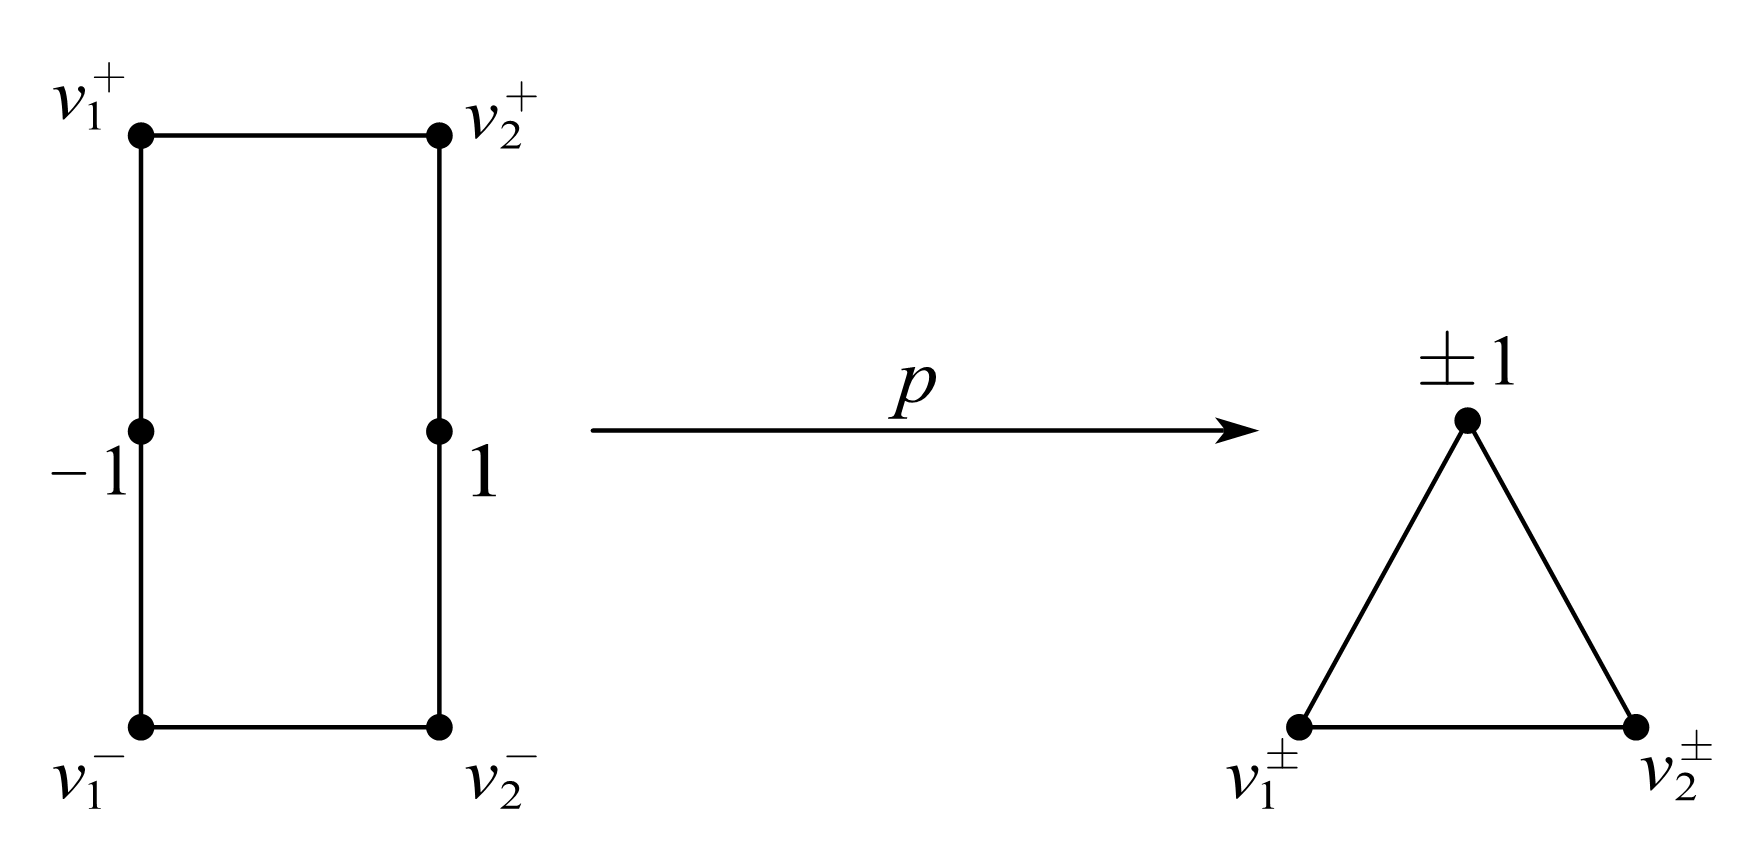
\includegraphics[width=0.3\linewidth]{figures/Sec13-2.png}
\end{figure}\\
那么对 $ e_\alpha^p\subset X^p\sm X^{p-1} $, 它落在 $ K $ 的一个开单形中, 即 $ \bar{e}_\alpha $ 可被 $ K $ 的子复形三角剖分. 因此, 对 $ H_p(\bar{e}_\alpha,\dot{e}_\alpha) $ 的计算可以归结为对单纯同调的计算. 我们称 $ H_p(\bar{e}_\alpha,\dot{e}_\alpha) $ 的生成元为一个\emph{基本闭链}.

\begin{Proposition}
	$ \partial : D_{p+1}(\RP^n)\to D_p(\RP^n) $ 在 $ 0\leqslant p=2k+1\leqslant n $ 时是将基本闭链 $ \times 2 $, (\textit{这一映射之后也直接记作 $ \times 2 $}), 当 $ p=2k $ 时 $ \partial=0 $.
\end{Proposition}
\begin{Proof}
	取 $ H_p(E_+^{p},\S^{p-1}) $ 中的一个基本闭链 $ \set{c_p} $, 那么 $ c_p\in Z_p(E_+^p,\S^{p-1}) $, 于是 $ \partial c_p $ 被 $ \S^{p-1} $ 承载. 构造
	\[
		\gamma_p=c_p+(-1)^{p-1} r_\sharp(c_p),
	\]
	这里 $ r $ 是对径映射, $ r_\sharp(c_p) $ 是 $ H_p(E_-^p,\S^{p-1}) $ 的生成元, 它被 $ \S^p $ 承载. 计算
	\[
		\partial\gamma_p=\partial c_p+(-1)^{p-1}r_\sharp(\partial c_p)=\partial c_p+(-1)^{p-1}(-1)^{p+1}\partial c_p=0.
	\]
	于是 $ \set{\gamma_p} $ 是 $ H_p(\S^p) $ 的生成元, 那么
	\begin{center}
		\begin{tikzcd}[row sep=small]
			H_p(\S^p) \arrow[r, "p_*"]        & H_p(\RP^p) \arrow[r, "j_*"]                 & {H_p(\RP^p,\RP^{p-1})}            \\
			\set{\gamma_p} \arrow[r, maps to] & \set{p_\sharp(\gamma_p)} \arrow[r, maps to] & \set{j_\sharp p_\sharp(\gamma_p)}
		\end{tikzcd}
	\end{center}
	注意到
	\begin{center}
		\begin{tikzcd}
			\S^p \arrow[r, "r"] \arrow[rd, "p"] & \S^p \arrow[d, "p"] \\
			 & \RP^n
		\end{tikzcd}
	\end{center}
	故有 $ p=pr $. 直接计算
	\[
		\begin{aligned}
			j_\sharp p_\sharp(c_p+(-1)^{p-1} r_\sharp(c_p))&=j_\sharp(p_\sharp(c_p)+(-1)^{p-1}p_\sharp r_\sharp(c_p))\\
			&=j_\sharp(p_\sharp r_\sharp(c_p)+(-1)^{p-1}p_\sharp r_\sharp(c_p))\\
			&=j_\sharp p_\sharp((1+(-1)^{p-1})c_p)
		\end{aligned}
	\]
	可知命题成立.\qed
\end{Proof}

\begin{Theorem}
	实射影空间 $ \RP^n $ 的同调群如下:
	\[
		\tilde{H}_p(\RP^{2n+1})=\begin{cases}
			\Z/2\Z & ,p=2k+1,0\leqslant k\leqslant n \\ \Z & ,p=2n+1 \\ 0 & ,\text{其他}
		\end{cases},\quad \tilde{H}_p(\RP^{2n})=\begin{cases}
			\Z/2\Z & ,p=2k+1,0\leqslant k\leqslant n \\ 0 & ,\text{其他}
		\end{cases}
	\]
	特别地,
	\[
		\tilde{H}_p(\RP^\infty)=\begin{cases}
			\Z/2\Z & ,p=2k+1, k\geqslant 0 \\ 0 &,\text{其他}
		\end{cases}
	\]
\end{Theorem}
\begin{Proof}
	直接考虑长正合列
	\begin{center}
		\begin{tikzcd}[column sep=small]
			D_{2n+1}(\RP^{2n+1}) \arrow[r, "0"] & D_{2n}(\RP^{2n+1}) \arrow[r, "\times 2"] & D_{2n-1}(\RP^{2n+1}) \arrow[r] & \cdots \arrow[r] & D_1(\RP^{2n+1}) \arrow[r, "0"] & D_0(\RP^{2n+1}) \arrow[r, "\id"] & \Z
		\end{tikzcd}
	\end{center}
	和
	\begin{center}
		\begin{tikzcd}[column sep=small]
			D_{2n}(\RP^{2n}) \arrow[r, "\times 2"] & D_{2n-1}(\RP^{2n}) \arrow[r, "0"] & D_{2n-2}(\RP^{2n}) \arrow[r] & \cdots \arrow[r] & D_1(\RP^{2n}) \arrow[r, "0"] & D_0(\RP^{2n}) \arrow[r, "\id"] & \Z
		\end{tikzcd}
	\end{center}
	即可.\qed
\end{Proof}

这同时说明了 $ \RP^{2n+1} $ 是可定向的, 但是 $ \RP^{2n} $ 不可定向.

相交于实射影空间的情形, 复射影空间的 CW 复形结构和同调群都更简单一些.

\begin{Proposition}
	$ X=\CP^n $ 是一个 CW 复形, 对 $ p\leqslant n $, $ X $ 恰有一个 $ 2p $--开胞腔, 且 $ X^{2p}=\CP^n $. 它没有任何奇数维开胞腔. 此时同调群的结果显而易见:
	\[
		H_p(\CP^n)=\begin{cases}
			\Z & ,p=2k, 0\leqslant k\leqslant n\\ 0 &,\text{其他}
		\end{cases}
	\]
\end{Proposition}
\begin{Proof}
	考虑这样的嵌入:
	\[
		\rho : \C^{n+1}\to\R^{2n+2},\qquad (z_1,z_2,\dots,z_{n+1})\mapsto(\Re z_1,\Im z_1,\dots,\Re z_{n+1},\Im z_{n+1}),
	\]
	并且在 $ \R^{2n+2} $ 上注意到 $ \norm{\rho(z)}=\norm{z} $, 于是它是一个同胚. 在后续的讨论中, 我们在合适的时候使用核是的空间.

	视 $ \CP^n $ 是 $ \C^\infty $ 的子集, 它可以看作 $ \S^{2n+1}/\S^1 $, 也即在 $ n+1 $ 维复球面 $ \S^{2n+1} $ 上定义这样的等价关系: 当 $ \abs{\lambda}=1 $, 也即 $ \lambda\in\S^1 $ 时,
	\[
		(z_1,z_2,\dots,z_{n+1},0,\dots)\sim(\lambda z_1,\lambda z_2,\dots,\lambda z_{n+1},0,\dots).
	\]
	记
	\[
		p : \S^{2n+1}\to\CP^n\cong\S^{2n+1}/\S^1,
	\]
	下面证明 $ p $ 是商映射. 为此只需 $ p $ 是闭映射. 设 $ A\subset\S^{2n+1} $ 是闭子集, 则 $ p^{-1}p(A)=l(\S^1\times A) $, 这里
	\[
		l : \S^1\times\S^{2n+1}\to\S^{2n+1},\qquad (\lambda,z)\mapsto\lambda z
	\]
	是一个自由作用(\textit{即没有不动点的作用}), 那么 $ l(\S^1\times A) $ 是紧集, 从而是闭的. 由此 $ p(A) $ 也是闭集, 这就说明了 $ p $ 是闭映射.

	考虑下面的作用:
	\begin{figure}[htbp]
		\centering
		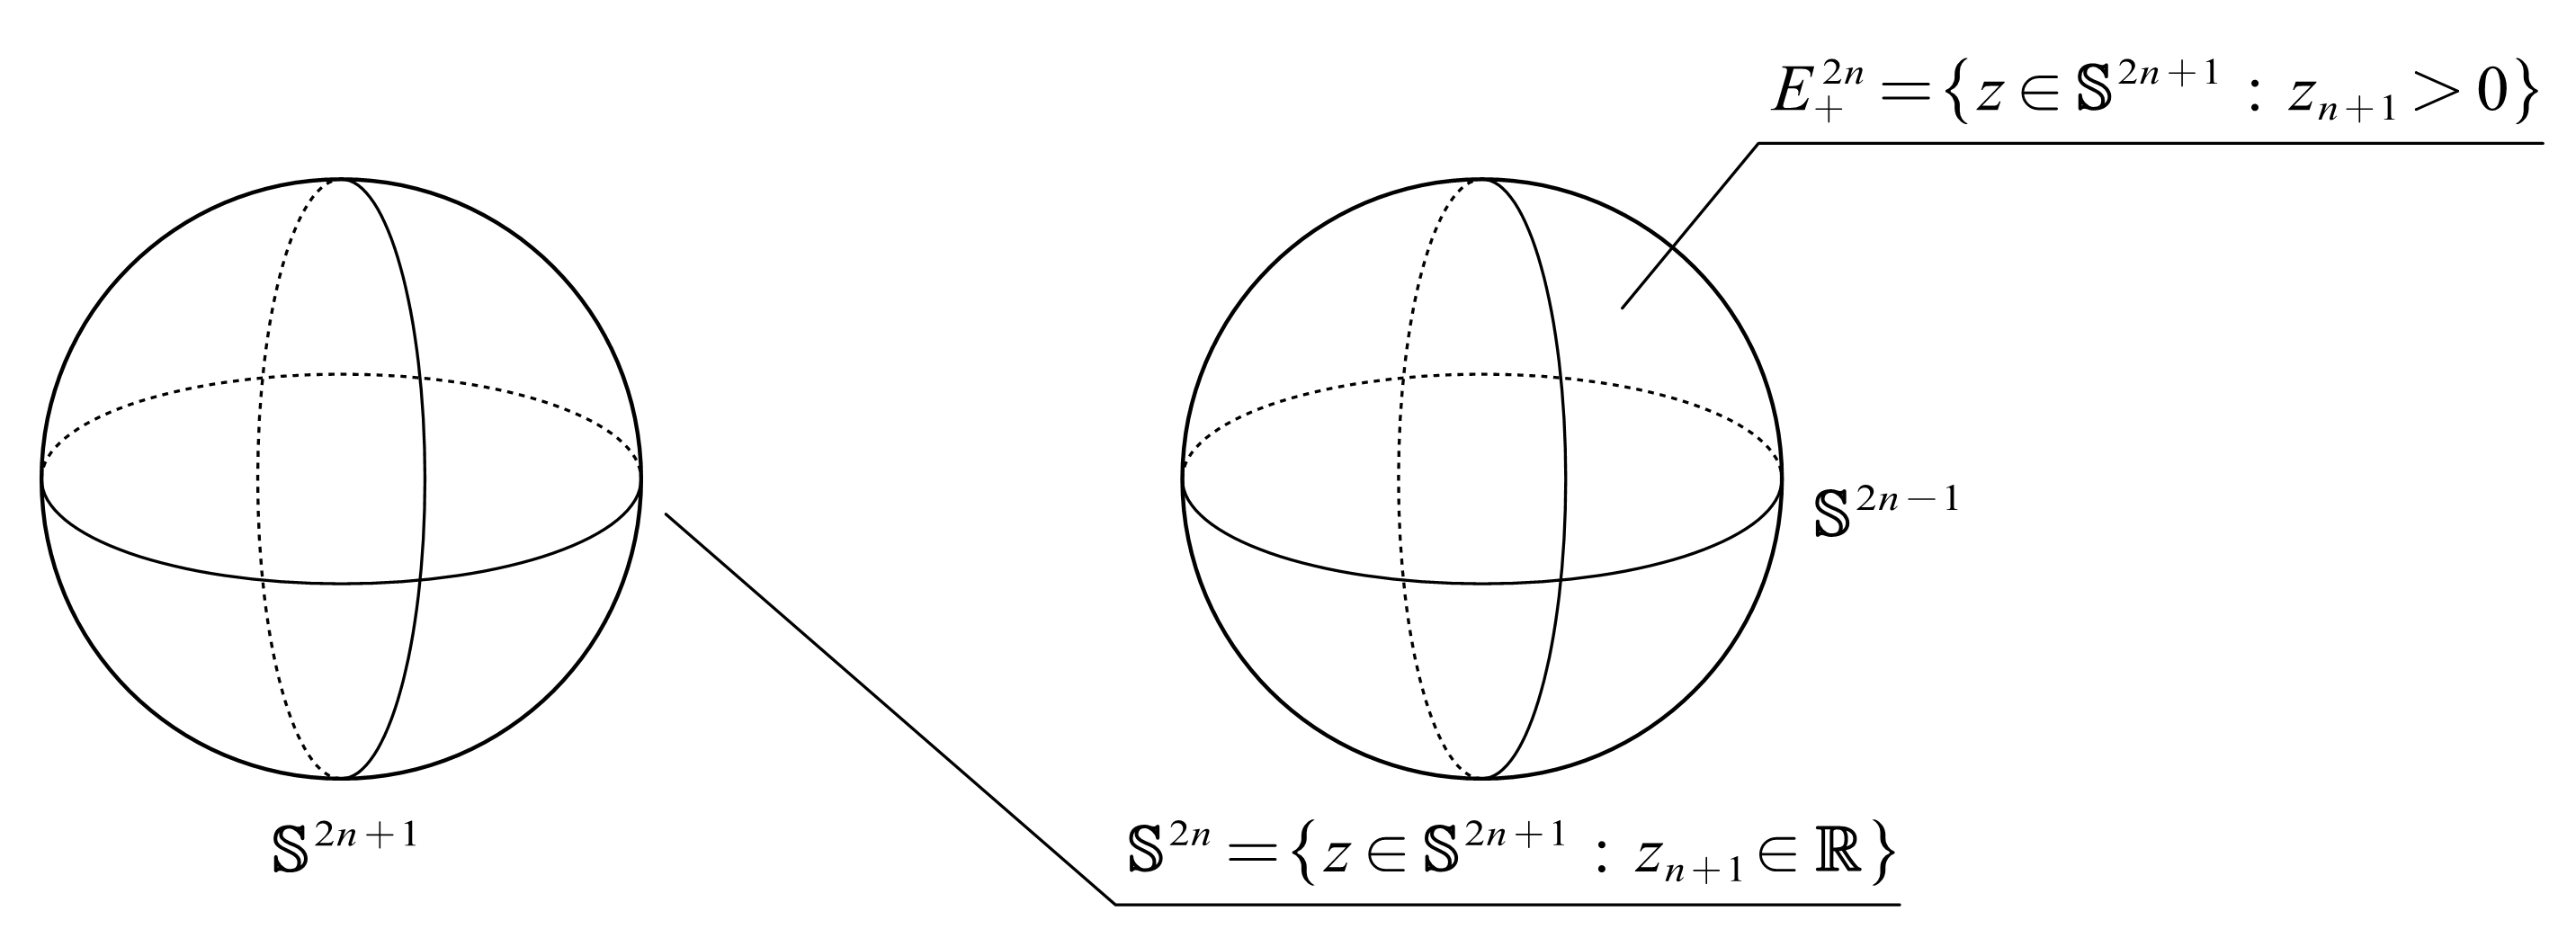
\includegraphics[width=0.75\linewidth]{figures/Sec13-3.png}
	\end{figure}\\
	只需证明
	\[
		p|_{\mathrm{Int}\,E_+^{2n}} : \mathrm{Int}\,E_+^{2n}\to\CP^n\sm\CP^{n-1}=:e_\alpha^{2n}
	\]
	是一个同胚即可.(\textit{这因 $ \S^{2n-1} $ 是复球面的复赤道})

	它是单的, 因对 $ z,z' $ 满足 $ p(z)=p(z') $, 存在 $ \lambda\in\S^1 $ 使得 $ z=\lambda z' $, 于是 $ z_{n+1}=\lambda z_{n+1}' $. 但 $ z_{n+1}>0 $, $ z_{n+1}'>0 $, 于是 $ \lambda>0 $. 而 $ \lambda\in\S^1 $, 只能 $ \lambda=1 $, 这即 $ z=z' $.

	它是满的, 因对任意 $ a\in e_\alpha^{2n} $, 存在 $ z\in\S^{2n+1}\sm\S^{2n-1} $, $ \abs{z}=1 $ 满足 $ z_{n+1}=r\me^{\imag\theta} $, 这里 $ r>0 $. 那么取 $ \lambda=\me^{-\imag\theta} $ 之后就有 $ \lambda z_{n+1}=r>0 $, 于是 $ \lambda z\sim z\in\mathrm{Int}\,E_+^{2n} $, 这即 $ p(z)=p(\lambda z)\in p(\mathrm{Int}\,E_+^{2n}) $.\qed
\end{Proof}